\documentclass{standalone}
\usepackage{tikz}
\usetikzlibrary{arrows.meta}
\tikzset{label/.style = {inner sep=1pt, fill=white}}
%\tikzset{nd/.style={circle, inner sep=0pt}}
\tikzset{nd/.style={inner sep=1pt}}
\tikzset{>=Latex}
\tikzset{arc/.style = {->, semithick, >=Latex}}
\begin{document}
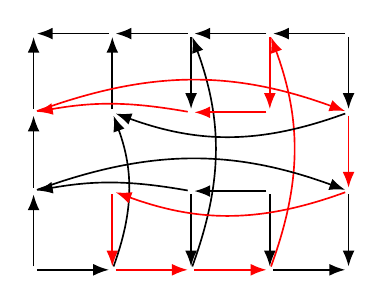
\begin{tikzpicture}

    \node[nd] (00) at (0,0) {};
    \node[nd] (01) at (0,1) {};
    \node[nd] (02) at (0,2) {};
    \node[nd] (03) at (0,3) {};
    \node[nd] (10) at (1,0) {};
    \node[nd] (11) at (1,1) {};
    \node[nd] (12) at (1,2) {};
    \node[nd] (13) at (1,3) {};
    \node[nd] (20) at (2,0) {};
    \node[nd] (21) at (2,1) {};
    \node[nd] (22) at (2,2) {};
    \node[nd] (23) at (2,3) {};
    \node[nd] (30) at (3,0) {};
    \node[nd] (31) at (3,1) {};
    \node[nd] (32) at (3,2) {};
    \node[nd] (33) at (3,3) {};
    \node[nd] (40) at (4,0) {};
    \node[nd] (41) at (4,1) {};
    \node[nd] (42) at (4,2) {};
    \node[nd] (43) at (4,3) {};

    \draw[arc] (00) to (10);
    \draw[arc,red] (10) to (20);
    \draw[arc,red] (20) to (30);
    \draw[arc] (30) to (40);
    \draw[arc] (00) to (01);
    \draw[arc] (01) to (02);
    \draw[arc] (02) to (03);

    \draw[arc] (43) to (33);
    \draw[arc] (33) to (23);
    \draw[arc] (23) to (13);
    \draw[arc] (13) to (03);
    \draw[arc] (43) to (42);
    \draw[arc,red] (42) to (41);
    \draw[arc] (41) to (40);

    \draw[arc,red] (11) to (10);
    \draw[arc] (10) to [out = 70, in=-70] (12);
    \draw[arc] (12) to (13);

    \draw[arc] (21) to (20);
    \draw[arc] (20) to [out = 70, in=-70] (23);
    \draw[arc] (23) to (22);

    \draw[arc] (31) to (30);
    \draw[arc,red] (30) to [out = 70, in=-70] (33);
    \draw[arc,red] (33) to (32);

    \draw[arc,red] (32) to (22);
    \draw[arc,red] (22) to [out = 170, in= 10] (02);
    \draw[arc,red] (02) to [out = 20, in=160] (42);
    \draw[arc] (42) to [out = -160, in=-20] (12);

    \draw[arc] (31) to (21);
    \draw[arc] (21) to [out = 170, in= 10] (01);
    \draw[arc] (01) to [out = 20, in=160] (41);
    \draw[arc,red] (41) to [out = -160, in=-20] (11);

 \end{tikzpicture}
\end{document}